\chapter{Wstęp}
\section{Cele i założenia projektowe}
Celem projektu było zapoznanie się z tematem uczenia maszynowego, a konkretnie z sieciami neuronowymi.
Realizacja projektu miała umożliwić zrozumienie zasady działania oraz porównanie wydajności sieci neuronowych używających propagacji wstecznej oraz wariantu o nazwie \textit{Extreme Learning Machines.}
\section{Wstęp teoretyczny}
Sieci neuronowe stanowią jedno z możliwych podejść do tematu uczenia maszynowego.
Są one modelowane na podobieństwo neuronów w mózgu, a zastosowanie znajdują między innymi w problemach klasyfikacji -- np. klasyfikacji stopnia złośliwości raka, tak jak to miało miejsce w projekcie.

Wzrost popularności zawdzięczają pojawieniu się szybszych komputerów oraz ogromnej ilości danych dostępnych do uczenia ich, co pozwoliło na zredukowanie wpływu głównych wad sieci neuronowych -- wolnego uczenia się oraz wymagania dużych zestawów danych uczących.
\subsection{Budowa sieci neuronowych}
Prosta sieć neuronowa może być zbudowana z trzech warstw neuronów:
\begin{itemize}
	\item{warstwy neuronów wejściowych,}
	\item{warstwy neuronów ukrytych,}
	\item{warstwy neuronów wyjściowych.}
\end{itemize}
Każda z warstw odbiera dane, a następnie po obliczeniu wartości funkcji aktywacji, przesyła dane do kolejnej warstwy.

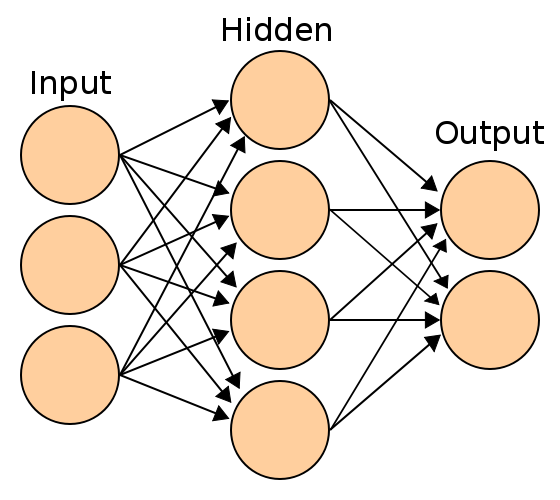
\includegraphics[scale=0.3]{img/model.png}